\usetikzlibrary{calc}
% 2007浙江理科19几何体,EA/DB垂直底面,M为AB中点
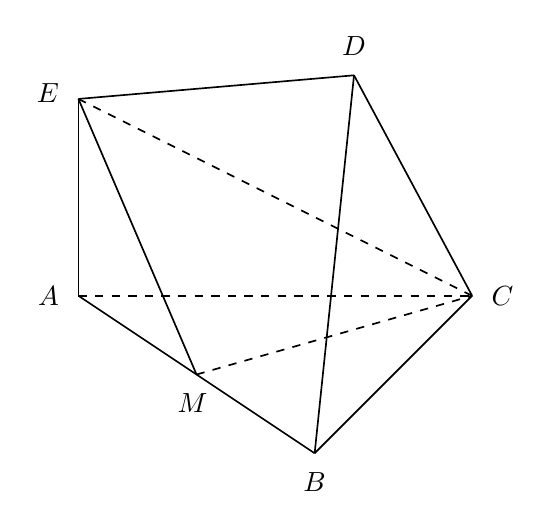
\begin{tikzpicture}[x=1cm,y=1cm,line width=0.6pt]
\coordinate (E) at (0.0,4.5);
\coordinate (A) at (0.0,2.0);
\coordinate (M) at (1.5,1.0);
\coordinate (B) at (3.0,0.0);
\coordinate (C) at (5.0,2.0);
\coordinate (D) at (3.5,4.8);
\draw[draw=black] (E)--(A);
\draw[draw=black] (E)--(D);
\draw[draw=black] (E)--(M);
\draw[draw=black] (D)--(B);
\draw[draw=black] (D)--(C);
\draw[draw=black] (B)--(C);
\draw[draw=black] (A)--(M)--(B);
\draw[draw=black,dashed] (E)--(C);
\draw[draw=black,dashed] (A)--(C);
\draw[draw=black,dashed] (M)--(C);
\node[anchor=east,font=\normalsize] at ($(E)+(-0.12,0.08)$) {$E$};
\node[anchor=east,font=\normalsize] at ($(A)+(-0.12,0)$) {$A$};
\node[anchor=north,font=\normalsize] at ($(M)+(-0.05,-0.12)$) {$M$};
\node[anchor=north,font=\normalsize] at ($(B)+(0,-0.12)$) {$B$};
\node[anchor=west,font=\normalsize] at ($(C)+(0.12,0)$) {$C$};
\node[anchor=south,font=\normalsize] at ($(D)+(0,0.12)$) {$D$};
\end{tikzpicture}
